% template.tex, dated April 5 2013
% This is a template file for Annual Reviews 1 column Journals
%
% Compilation using ar-1col.cls' - version 1.0, Aptara Inc.
% (c) 2013 AR
%
% Steps to compile: latex latex latex
%
% For tracking purposes => this is v1.0 - Apr. 2013

\documentclass{style/ar-1col}
\usepackage[utf8]{inputenc}
\usepackage{url}
\usepackage[numbers]{natbib}
\bibliographystyle{bib/ar-style6}
\usepackage{multirow}
\usepackage{todonotes}
%\usepackage{caption}
\usepackage{subcaption}
\usepackage{graphicx}
\usepackage{comment}
\usepackage{tabularx}
\usepackage{tablefootnote}

% Set up ORCiD. See <https://tex.stackexchange.com/a/445583>
\begin{comment}
\usepackage{scalerel}
\usepackage{tikz}
\usetikzlibrary{svg.path}
\definecolor{orcidlogocol}{HTML}{A6CE39}
\tikzset{
  orcidlogo/.pic={
    \fill[orcidlogocol] svg{M256,128c0,70.7-57.3,128-128,128C57.3,256,0,198.7,0,128C0,57.3,57.3,0,128,0C198.7,0,256,57.3,256,128z};
    \fill[white] svg{M86.3,186.2H70.9V79.1h15.4v48.4V186.2z}
                 svg{M108.9,79.1h41.6c39.6,0,57,28.3,57,53.6c0,27.5-21.5,53.6-56.8,53.6h-41.8V79.1z M124.3,172.4h24.5c34.9,0,42.9-26.5,42.9-39.7c0-21.5-13.7-39.7-43.7-39.7h-23.7V172.4z}
                 svg{M88.7,56.8c0,5.5-4.5,10.1-10.1,10.1c-5.6,0-10.1-4.6-10.1-10.1c0-5.6,4.5-10.1,10.1-10.1C84.2,46.7,88.7,51.3,88.7,56.8z};
  }
}
\newcommand\orcidicon[1]{\href{https://orcid.org/#1}{\mbox{\scalerel*{
\begin{tikzpicture}[yscale=-1,transform shape]
\pic{orcidlogo};
\end{tikzpicture}
}{|}}}}
\end{comment}

\newcommand\orcidicon[1]{\href{https://orcid.org/#1}{$^\sigma$}}

\usepackage{hyperref} %<--- Load after everything else

% Define a way to rotate table headings. See
% <https://tex.stackexchange.com/a/98439>
\newcommand*\rot{\rotatebox{90}}

% Define a way to cram two lines into a non-paragraph cell
% See <https://tex.stackexchange.com/a/132661>
\newcommand{\twoline}[2]{\vtop{\hbox{\strut #1}\hbox{\strut #2}}}

\listfiles

\setcounter{secnumdepth}{4}

% Metadata Information
\jname{Xxxx. Xxx. Xxx. Xxx.}
\jvol{AA}
\jyear{YYYY}
\doi{10.1146/((please add article doi))}


% Document starts
\begin{document}

\newcommand{\shorttitle}{Pangenome graphs}
\newcommand{\firstauthorlastname}{Eizenga}

% Page header
\markboth{\firstauthorlastname\ et al.}{\shorttitle}

% Title
\title{\shorttitle}


%Authors, affiliations address.
\author{%
  Jordan M \firstauthorlastname$^1$\orcidicon{0000-0001-8345-8356},
  Adam M Novak$^1$\orcidicon{0000-0001-5828-047X},
  \\
  Jonas A Sibbesen$^1$\orcidicon{0000-0002-5528-0236},
  Simon Heumos$^2$\orcidicon{0000-0003-3326-817X},
  \\
  Ali Ghaffaari$^{5,6,7}$,
  Glenn Hickey$^1$,
  Xian Chang$^1$,
  \\
  Josiah D Seaman$^{3,4}$\orcidicon{0000-0003-2374-630X},
  Robin Rounthwaite$^1$\orcidicon{0000-0002-0264-7487},
  Jana Ebler$^{5,6,7}$,
  Mikko Rautiainen$^{5,6,7}$\orcidicon{0000-0003-2971-267X},
  \\
  Shilpa Garg$^{8,9,10}$,
  Benedict Paten$^1$\orcidicon{0000-0001-8863-3539},
  \\
  Tobias Marschall$^{5,6}$\orcidicon{0000-0002-9376-1030},
  Jouni Sir\'{e}n$^1$\orcidicon{0000-0001-5828-4139},
  \\
  and Erik Garrison$^{*1}$\orcidicon{0000-0003-3821-631X}
\affil{\tiny$^1$Genomics Institute, University of California Santa Cruz, Santa Cruz, CA, USA, 95064}
\affil{\tiny$^2$Quantitative Biology Center, University of Tübingen, Tübingen, Germany, 72076}
\affil{\tiny$^3$Royal Botanic Gardens Kew, Richmond, UK, TW9 3AB}
\affil{\tiny$^4$Queen Mary University of London, London, UK, E1 4NS}
\affil{\tiny$^5$Center for Bioinformatics, Saarland University, Saarbr\"{u}cken, Germany, 66123}
\affil{\tiny$^6$Max Planck Institute for Informatics, Saarbr\"{u}cken, Germany, 66123}
\affil{\tiny$^7$Saarbr\"{u}cken Graduate School for Computer Science, Saarbr\"{u}cken, Germany, 66123}
\affil{\tiny$^8$Department of Genetics, Harvard Medical School, Boston, MA 02215}
\affil{\tiny$^9$Department of Data Sciences, Dana-Farber Cancer Institute, Boston, MA 02215}
\affil{\tiny$^{10}$Department of Biomedical Informatics, Harvard Medical School, Boston, MA 02215}
\affil{\tiny$\sigma$ORCID identifier hyperlinks}
\affil{\tiny$^*$email: erik.garrison@ucsc.edu}
}

%Abstract
\begin{abstract}
  Improved sequencing technology lets us collect whole genome assemblies of high quality from many individuals, which opens the possibility of working with a pangenome that represents the total genomic information in a species.
  Many recently-developed methods use pangenome reference systems as precise bases for bioinformatic analyses.
  These methods use compressed, often graph-based, and sometimes approximate models to implement algorithms for sequence alignment, visualization, functional genomics, and association studies at the scale of large eukaryotic pangenomes.
  Although sequence graphs feature prominently in these methods, most methods focus on communicating results in the frame of a linear reference genome, suggesting that linear reference representations will remain relevant into the near future.
  However, graphical pangenomes can work harmoniously with multiple linear reference systems, and so we expect them to unify and build upon standard reference genomes, rather than replacing them.
\end{abstract}

%Keywords, etc.
\begin{keywords}
genome graph, variation graph, graph, pangenome, reference
\end{keywords}
\maketitle

%Table of Contents
%\tableofcontents

\section{Introduction}

A \emph{pangenome} models the full set of genomic elements in a given species or clade.
Pangenomics thus stands in contrast to standard genomics by emphasizing the sum total of available genomic information over a particular consensus model of the genome.
By considering the pangenome during bioinformatic analyses, researchers can hope to remove bias towards any specific genome or haploid genome model that might occur during diverse stages of data processing.
%, analyse also minor alleles inevitably missing from such linear models, and incorporate information about genomic variation directly into their study.
%Pangenomic reference systems thus e single canonical version of the genome of a given species, but a widely-represenative collection of sequences.

This concept has been essential to microbiology, where genomic plasticity and diversity have made a pangenomic perspective indispensable \cite{Vernikos2015}.
Usually, these analyses focus on the presence or absence of genes from given strains and the determination of a core (commonly present) and accessory (frequently absent) pangenome \cite{page2015roary}.
Pangenomic techniques have also been applied outside of microbiology, such as in species contexts where genomes are small and often homozygous \cite{cao2011whole}, or in the publication or analysis of collections of novel sequences from a single species \cite{gao2019tomato,Ou_2018}.
In recent years, reduced sequencing and \emph{de novo} assembly costs have supported the discovery of significant levels of large-scale genomic variation in many eukaryotic species, including humans \cite{sudmant2015integrated,Hehir-Kwa2016-hb,chaisson2018multi,Audano_2019}, arabidopsis \cite{alonso2016arabidopsis}, brewer's yeast \cite{yue2017contrasting}, and the fruit fly \cite{chakraborty2018hidden}.

%These trends encourage the application of pangenomic methods to settings where more than one individual is being analyzed
These observations have yet to result in a major change to standard approaches to genomics.
Although there is wide interest in generalizing basic bioinformatic operations to use a pangenomic reference model \cite{computational2016computational}, today, most ``high-throughput'' analyses of large genomes still depend on comparison to a single reference genome.
This expedient and conservative approach has its merits, but will become untenable with the development of true pangenomic references for humans \cite{Church2015-vt} and other model organisms.
%But, to be a true replacement for resequencing, methods based on reference pangenomes must provide precise resolution of variants of all scales. %, and they must support efficient pangenomic generalizations of many standard bioinformatic approaches.

Here, we consider a new class of methods that approach the pangenome with precision, often at the resolution of single base pairs.
Unlike widely-applied pangenomic methods that consider genes as their fundamental unit, these precise pangenomic methods support the interrogation of collections of genomes and their relationships at any level of resolution.
They envision pangenomic analyses based on the full complement of DNA in the individuals under analysis, and aim to support downstream inference over variants of all types and scales.
%, including small variation such as SNPs and indels in the same context as large structural variants gene gain or loss.

Scaling such techniques to operate on eukaryotic pangenomes has required significant effort in the development of new data models and algorithms.
Solutions to this problem are varied, but they often rely on graph data structures that both compress a collection of genomes and express relationships between them.
Not all methods expose this data structure as a coherent reference system.
They may instead use it internally to improve performance of a standard bioinformatic operation.
Even different graph-based pangenomic models are not necessarily equivalent and may have distinct strengths and weaknesses in terms of representing certain kinds of genomic variation.

%Although these limitations have appeared necessary to scale precision pangenomics to eukaryotic genomes, new algorithms and approaches for the construction and interrogation of pangenome graphs demonstrate that generic models can be scalable.
%These results imply the possibility of simplifying and even expediting many bioinformatic analyses through the use of pangenomic reference systems and algorithms.

\subsection{Resequencing scales genome inference}

Genomics research depends on our ability to see the relationships between genomes.
In an earlier era, it was feasible to relate all of an experiment's sequences to each other, typically using multiple sequence alignment.
These analyses were effectively pangenomic. 
%In the early days of genomics, when the cost of sequencing was high, expensive algorithms would be applied to relate all sequences in a given experiment to all others, typically yielding multiple sequence alignments.
%These analyses were thus effectively pangenomic, in their unified representation of all the genomic information in the analysis.
Increasing data scales have made such approaches prohibitively costly.
Instead, high-quality genome assemblies and high-throughput sequencing have encouraged \emph{resequencing} methodologies, wherein reads from each sample are aligned to a single reference genome.
State of the art resequencing pipelines can analyze tens of thousands of genomes \cite{Poplin_2017}, but only by relating each genome to a single common reference sequence.

\subsection{Resequencing implies reference bias}

Although efficient and conceptually simple, resequencing has a significant limitation.
The relationships between genomes are only visible for those sequences that are similar enough to the reference genome to be alignable.
%Significant variation between a new genome and the reference genome may be rendered invisible, or apparently less frequent, by the reference bias inherent in alignment.
This effect is known as \emph{reference bias}.
It is certainly strongest for structural variation or sequences that are absent from the reference system \cite{sudmant2015integrated}, but it can be relevant even for SNPs, which cause problems in alleles specific expression (ASE) quantification \cite{Castel2015-ef} and in the analysis of ancient DNA \cite{zhou2017antcaller}.
Given that this bias shapes the methods that we use to establish models of the truth \cite{zook2014integrating}, it will be difficult to evaluate without paradigmatic change in our analysis techniques.
%JME: This sentence seems basically redundant with the one two sentences back. I see that you're citing pangenomic methods instead of traditional ones, but you seem to be making basically the same point. 
%Recent studies have applied variation-aware sequence alignment methods to show that this bias affects even the detection of small variation \cite{eggertsson2017graphtyper,Garrison_2018,Kim_2019}, and that these methods can be used to mitigate its effect on the study of ancient DNA \cite{martiniano2019removing} and RNA sequencing data \cite{Miao2018-ps,Liu_2018}.

\subsection{Human pangenomics}

Estimates based on short read sequencing data have placed the human pangenome at between 1\% \cite{li2010building} and 10\% \cite{sherman2019assembly} larger than the the GRCh38 human reference assembly.
Others have demonstrated up to several Mbp of sequence are present in each new individual and not in the reference \cite{Hehir-Kwa2016-hb,Steinberg_2016,Audano_2019}.
Although these estimates vary based on the author's definition of what constitutes novel sequence or allelic variation, we should expect them to rise as we consider larger cohorts of humans and improve our ability to ascertain variants in repeat-rich genomic regions.
In particular, we might gain greater insight into the extent, placement and significance of novel sequences when they are discovered in whole genome telomere-to-telomere assemblies constructed from long single-molecule sequencing data \cite{miga2019telomere,Langley_2019}.

%Efficiently relating new sequences to such rich data resources will require the application of new kinds of resequencing and new models for bioinformatic analysis that support the inference of sensitive all-to-all relationships between large collections of large genomes.
%The genomics community is today working to determine what kinds of data models will allow researchers to fully exploit pangenomic data from humans and other species.
%Much attention has been given to the type of data structure which

%In addition to allowing the use of pangenomes in genome inference, the decreasing cost of whole genome assembly suggests that a new problem will arise in comparing whole genomes to each other.
%This issue of whole genome alignment or comparison suggests an end to the dominance of resequencing based tools, and implies the need for greater focus on methods that can efficiently process and report on whole assemblies.




\section{Building pangenomic models}

\subsection{Constructing graphs} 

A linear genome is essentially a simple genome graph without any integrated genetic variation. 
More complex graphs can be constructed by inserting genetic variation as alternative paths in the linear genome, or can be constructed straight from \textit{de novo} assemblies. 
The primary advantage of including variation information in a genome graph---either by modifying a linear genome or by assembling a graph \textit{de novo}---is that the resulting genome graph conserves most or all of the sequence diversity present in the input assemblies. 
As we'll see in the algorithms below, a graph's utility is frequently measured in terms of its ability to use that diversity for effective sequence mapping and variant calling, and the improved representation of genes specific to individual populations.

\subsubsection{\textit{De novo} graph construction}
\todo{This section could be written at a higher level with more compare/contrast.}

The \texttt{vg} tool offers multiple graph construction algorithms, including the \textit{de novo} assembly algorithm MSGA (Multiple Sequence to Graph Aligner) \cite{Garrison_2018,Novak_2017a}. 
MSGA implements a progressive alignment strategy.
Initially, the graph is composed of any one sequence of the set of input sequences.
Each subsequent sequence is inserted into the current iteration of the graph, until the graph contains all the sequences from the input.
This algorithm is attractive because it only uses tools already present in \texttt{vg}, but the resulting graph is dependent on the order that the sequences were added.
In addition, the algorithm uses a large amount of working memory, which makes working with large populations of genomes untenable.

Seqwish\footnote{\url{https://github.com/ekg/seqwish}}, another \textit{de novo} construction algorithm in the \texttt{vg} ecosystem, was developed to address the weaknesses of MSGA.
Seqwish losslessly converts sets of pairwise alignments between sequences into a variation graph.
Input sequence alignments are usually all-to-all, although it's not required.
The algorithm constructs the graph by identifying chains of sequences that align together, which are then linked together to form walks through the graph.
By first implementing a disk-backed sort of the alignment and sequence inputs, the graph can be constructed in relatively low memory compared to the input sequence.
In a comparison of seqwish to MSGA on the challenging-to-sequence region Major Histocompatibility Complex (~5Mb), seqwish used several times less RAM than MSGA, but had to save 12 GB of intermediate files during construction \todo{Where is this comparison documented? It's not described in the seqwish README.}.


Novograph's algorithm also constructs graphs directly from assembly contigs without the need to integrate sequence information from a linear genome, although it requires a linear reference to determine the relative location of the contigs before integrating them into a graph \cite{Biederstedt2018}. 
The algorithm first computes a global pairwise alignment to determine the approximate placement of each input contig, which it uses to perform an approximate global multiple sequence alignment between all input contigs and the reference genome.
This identifies homology relationships between the input sequences and the reference genome.
The contigs are then merged at positions that are both homologous and sequence-identical to create a directed acyclic graph.

 
HUPAN, a pangenome analysis pipeline for human genomes, is a recently developed tool for assembling pangenome graphs \cite{Duan_2019}. 
To demonstrate the application of their tool, \citep{Duan_2019} identified several novel genes in the genomes of a set of Chinese individuals.
Pangenomes are graph-like in that they consist of a ``core genome'' containing genes present in all individual genomes and the ``distributed genome,'' which contains genes existing only in a subset of individuals.
That is, genes in the distributed genome must be absent or at least one individual.
The combination of core genome and distributed genome constitutes a genome graph because the location of distributed genes are marked in relation to coordinates in the core genome.\todo{is this true? I'm unclear how HUPAN constitutes a graph genome.}

HUPAN construction is reference genome-oriented.
For each individual in the population of interest, sequenced reads are assembled \textit{de novo} into contigs.
These contigs are then aligned to the reference genome.
Because some of the genetic sequence in the population isn't represented in reference, there are some reads that align only partially or not at all.
These are pooled, and aligned all-to-all.
After filtering to remove non-human sequences, the pangenome can be constructed by merging the now-connected partially- and fully-unaligned sequences with the reference genome.

\texttt{vg} also offers tools for constructing a genome graph using linear genomes, such as the Cactus progressive aligner \cite{Garrison_2018}.

\todo{Do we have a good publication detailing how Cactus graphs are constructed? Are there other \texttt{vg} algorithms I'm missing?}

\subsubsection{Graph construction based on existing linear genomes}

GenomeMapper was the first major tool to use a reference genome graph \cite{Schneeberger_2009}.
The genome graph was constructed by indexing, and then merging, a population of genomes. 
The index, which is effectively a compilation of the locations of all sequence signatures of 5 to 13 bp in length, guided the alignment process by offering an easy-access tool for identifying sets of similar substrings that are close to one another between genomes. 
The GenomeMapper graph demonstrated access to polymorphisms that were otherwise unavailable in a linear reference.

\texttt{vg}'s MSGA can also be used for constructing a graph based on linear input genomes, instead of assembly contigs.
Starting with a graph composed entirely from a full linear genome, MSGA constructs a more complex graph by using the same progressive align-andintegrate strategy as is used for \textit{de novo} graph construction. \todo{citation needed}

\subsubsection{Graph genome coordinates}

Offset coordinates make it easy to unambiguously refer to any position or interval in a linear genome.
Offset-based coordinate systems typically have two components: name of the chromosome, and distance in nucleotides (nt) from the chromosome's start.
For example, ``chr14:100k'' would be on chromosome 14, 100,000~nt from the start.
Because genome graphs can include multiple walks of varying length, however, offset coordinates in a graph would vary depending on which path was taken.
To resolve this problem, one graph-based coordinate system uses a similar offset-based format, except that the name of the chromosome is replaced with name of the \emph{DNA region}; and similarly distance in nt from the \emph{region's} start \cite{Rand_2016}. 
The DNA region can be the chromosome itself, if the coordinate is on the linear backbone of the graph.
In regions with alternate paths, however, the DNA region would be the alternative allele ID in the graph.
For example, a coordinate for an alternate path in the IGH region could be ``IGH-alt1:350'', which would be 350~nt from the designated starting point of the alt path.
Intervals in a graph are defined by a list of the genomic regions the interval passes through, e.g. ``chr14:100, IGH-alt1, SERPIN-alt1, chr14:150m''.
This coordinate system was chosen because it at least partially satisfies the four criteria of \citeauthor{Rand_2016} by providing good:
\begin{itemize}
    \item \emph{Readability}: it is relatively easy for humans to interpret.
    \item \emph{Backward compatiblity}: adding more variants to the graph doesn't invalidate previously established coordinate points in the graph.
\end{itemize}
It also provides acceptable:
\begin{itemize}
    \item \emph{Spatiality}: nearby bases frequently have similar coordinates, within a DNA region or within similarly named regions.
    \item \emph{Monotonicity}: coordinates increase gradually the further they are from the start of the chromosome, within a DNA region.
\end{itemize}

\todo{Where are we going with this? Are we just saying that offset based coordinates are a good idea? Are we going to talk about whether/how tools like \texttt{vg} use them?}

\subsubsection{Measuring graph utility}

Because \texttt{vg} provides an integrated toolkit for constructing, manipulating, and using genome graphs, it's a tool well-suited for comparing the efficacy of different genome graph construction techniques \cite{Novak_2017, Garrison_2018}.
In the paper ``Genome Graphs'', \citeauthor{Novak_2017a}\ compared different graph constructions based on their utility in read mapping, variant calling, and general graph character \citep{Novak_2017a} \todo{Does it really make sense to lean so heavily on our own unreviewed, unpublished manuscript in a review?}.
They found that genome graphs in general provide superior read mapping and variant calling to their linear counterparts, and that different construction approaches varied greatly even within each region of the genome.
To quantify this variability, they proposed three normalized graph metrics.
 \emph{Graph compression} is the length of primary reference sequence divided by the sum of the length of the nodes in the graph.
It essentially measures the quantity of alt path sequence represented in the graph with respect to the size of the reference.
The \emph{(base) degree} of the graph measures how much branching occurs in the graph, and the \emph{cut width} measures apparent sequence rearrangement \todo{We don't have any evidence to support these being useful or accepted metrics, though.}.


In the same study, \citeauthor{Novak_2017a}\ demonstrated that their graphs improved mapping precision when more polymorphisms were added to the graph.
As they pointed out, this is a potentially surprising result: they originally thought that adding more sequences similar to the read's target would reduce the likelihood of the read mapping to the correct region.
Instead, adding known variants helped the mapping algorithm distinguish their true mapping location from other, paralogous sequences \citep{Novak_2017a}.

\subsubsection{Improving graph utility with FORGe: A tool for prioritizing variants for graph genomes}

Adding more variants to the graph doesn't always improve mapping precision, however.
FORGe is a tool for modeling the effects of adding a variant to the graph \cite{Pritt_2018}. 
The primary benefit of adding a variant to the graph is that it increases the graph's representation of sequence diversity.
Without variance in the graph, reads with significant sequence dissimilarity from the linear genome won't be mapped to the correct region, or won't be mapped at all.
Sometimes, however, adding a variant can reduce alignment accuracy by increasing the ambiguity of similar sequences already in the graph.
In addition, adding variants to the graph can increase the cost of storing and querying the genome index.
To predict the effects of adding a variant, FORGe scores variants based on their frequency in a population, its proximity to other variants, and how it increases/decreases repetitive sequence in the genome.
It can then output a list of top-scoring variants for use in a graph aligner.
\todo{How do we square the results showing FORGe is needed with the results from our unpublished Graph Genomes manuscript? We don't do that work here.}


\subsection{Indexing genome graphs}

A \emph{text index} maps query strings to their occurrences in the indexed text.
The occurrences are typically reported as a list of starting positions, from which one can easily determine the substrings matching the query.

Indexing the sequences encoded in a graph is more involved.
The number of $k$~bp paths often grows exponentially in $k$, and the number of distinct $k$-mers encoded as path labels may also grow exponentially.
Indexing or even enumerating all $k$-mers in the graph may be infeasible for reasonable values of $k$, and if the starting position of the occurrence reported by the index is in a complex region of the graph, there may be an exponential number of $k$~bp paths to investigate.

In practice, indexes for genome graphs must make trade-offs not encountered in text indexes.
In order to limit the exponential growth, the index may only support relatively short query strings.
Some indexes (e.g.\ \cite{Siren_2014}) support longer queries by doing extensive preprocessing.
In other indexes (e.g.\ \cite{Thachuk_2013,Huang_2013,Maciuca_2016}), queries mapping to complex graph regions can be slow.
Instead of indexing the entire graph, the index may only contain $k$-mers from a simplified graph, or from specific paths of the graph.
While finding the path matching the query may be expensive in some cases, indexes typically save space by only reporting the starting position of the match.

\subsubsection{Indexing sequences using a graph}

The FM-index \cite{Ferragina_2005} is a text index, based on the Burrows--Wheeler transform (BWT) \cite{Burrows_1994}, that is frequently used with DNA sequences.
One variant of the FM-index, the RLCSA \cite{Maekinen_2010}, run-length encodes the BWT, allowing it to store and index a collection of similar sequences space-efficiently.
\citeauthor{Huang_2010}\ \cite{Huang_2010} observed that if we know a good global alignment of the sequences, we can use that information to make the index both smaller and faster.
\citeauthor{Na_2016}\ \cite{Na_2016,Na_2018} developed this approach further in their FM-index of alignment.
While the articles do not mention it, both \citeauthor{Huang_2010}\ and \citeauthor{Na_2016}\ use the graph induced by the alignment as a space-efficient representation of the sequences.

\subsubsection{Indexing acyclic graphs}

One class of graph indexing methods supports only acyclic graphs, often represented as directed acyclic graphs (DAGs).
This constraint can exist either because the acyclicity of the graph provides guarantees that simplify the problem, or because incedental features of the method's software implementation preclude use on cyclic graphs.
One common class of DAGs, here called \emph{VCF graphs}, represents each contig as a mostly linear run of graph nodes, branching to allow only for substitutions and possibly insertions and deletions.
\todo{``VCF graph'' is a placeholder; is there a better term for this shape?}

GenomeMapper \cite{Schneeberger_2009} was the first graph-based read aligner.
It builds a VCF graph from a reference sequence and a set of variants.
To index the graph, GenomeMapper uses a simple hash-based $k$-mer index, with $k \le 13$ to limit memory usage.

GCSA \cite{Siren_2014} was the first attempt to use the BWT with graphs.
It either takes a prebuilt DAG or generates one from a multiple alignment of sequences.
GCSA then applies a number of graph transformations that preserve the language, or set of end-to-end sequences, until the nodes can be unambiguously sorted by the labels of the paths starting from the node.
When the complexity of the graph is sufficiently low, these transformations are reasonably fast and do not increase the size of the graph significantly.
However, a phase transition happens at a certain threshold, and the transformed graph quickly becomes too large to handle above the threshold.

BWBBLE \cite{Huang_2013} is a BWT-based representation for VCF graphs.
Simple substitutions are encoded in the sequence using IUPAC codes, and the sequence is indexed using a normal FM-index.
Because each base can be encoded using 8 different characters, the search branches at every base to cover all possible characters which admit the base searched.
In practice, most branches quickly run out of results and can be pruned from the search.
Insertions and deletions produce separate sequences, with selected amount of context around the variant.
The length of this context is an effective upper bound for query length.

The vBWT \cite{Maciuca_2016} took another approach to using the BWT for indexing VCF graphs.
It encodes variants as \texttt{(ref|alt1|alt2|\dots)} in the sequence.
When the search encounters a variant, it must branch to handle each allele separately.
Both BWBBLE and vBWT trade faster index construction for slower queries.
However, a combination of IUPAC codes for substitutions, the vBWT approach for other variants, and a $k$-mer index for matching the first 5--10 bases, is faster than either of the originals \cite{Buechler_2019}.

\subsubsection{General graphs}

Some text indexes are based on Lempel--Ziv parsing or context-free grammars.
These indexes first find partial matches between the query string and the indexed phrases and then combine the partial matches into full matches using two-dimensional range queries.
In the hypertext index \cite{Thachuk_2013}, each node is a separate phrase.
Queries mapping to a single node or crossing a single edge can be matched efficiently, while finding mappings to complex graph regions can be slow.

\citeauthor{Bowe_2012}\ \cite{Bowe_2012} used techniques similar to GCSA for representing de~Bruijn graphs.
If the graph transformations used in GCSA construction are stopped after $i$ steps, the resulting graph is equivalent to an order-$2^{i}$ de~Bruijn graph.
This de~Bruijn graph can be used to approximate the original graph.
There are no false negatives, but matches longer than $2^{i}$ may be false positives.
By using this approach, GCSA2 \cite{Siren_2017} attempts to support fast queries in arbitrary graphs.

GCSA2 faces the same issues with complex graphs as GCSA.
In practice, most graphs must be simplified before they can be indexed.
Typical simplifications include removing high-degree nodes and complex regions from the graph and replacing them with the reference sequence.
If a collection of haplotypes is available, the removed regions can be replaced with new subgraphs that contain separate paths for each distinct local haplotype \cite{Siren_2019}.
This way, the index contains all $k$-mers from the haplotypes, while usually missing $k$-mers from their recombinations.

\subsubsection{Indexing graphs using sequences}

Instead of attempting to index the entire graph, it is often sufficient to index only selected paths in it.
CHOP \cite{Mokveld_2018} takes the paths corresponding to haplotypes and breaks them into smaller pieces.
The distinct pieces form an artificial linear reference, which can be used with any read aligner.
The process guarantees that any substring of the haplotypes of length $k$ is also a substring of one of the pieces.
As with BWBBLE, $k$ represents an effective upper bound for query length.

The ``Pan-genome [sic] Seed Index'' (PSI) \cite{Ghaffaari_2019} follows a similar approach with artificial paths.
Instead of using haplotypes, PSI uses a greedy algorithm to find a set of paths that covers as many $k$~bp windows in the graph as possible.
An index using these paths alone already works well in practice.

When a fully sensitive index is needed, PSI can reverse the role of the query strings and the graph.
While complex graph regions may contain an excessive number of $k$-mers, the reads mapping to them only contain a limited number of $k$-mers.
By indexing a batch of reads and searching for the complex regions in that index, all mappings of the query strings to the graph can be found with reasonable resources.


\subsection{Other population-ish succinct data structures}
% Erik

\subsubsection{de Bruijn}

% BOSS: \cite{Bowe_2012} (\cite{Roedland_2013} is similar)

\subsubsection{VCFs / genotype calls / haplotypes / binary matrices}

\subsubsection{gPBWT, GBWT}

% Jouni: We should at least include this


\subsubsection{Alignments / collections of strings}

% Jouni: We probably don't have space for this.




\section{Relating new information to the pangenome}

\subsection{Visualization}
% Adam

Once one has constructed a graph pangenomic model, one might want to look at it.
A number of tools have been developed for this purpose.

Bandage (\textbf{B}ioinformatics \textbf{A}pplication for \textbf{N}avigating \textit{\textbf{D}e novo} \textbf{A}ssembly \textbf{G}raphs \textbf{E}asily) \citep{Wick_2015} is one of the most popular \citep{Mikheenko_2019}.
Originally designed for working with bacterial assembly and meta-assembly graphs \citep{Wick_2015}, it supports a wide range of formats and graph  paradigms.
It can be effectively used for interactively visualizing and exploring subregions of human-scale pangenome graphs \citep{Garrison_2019}, but its shortcomings become apparent at larger scales or with higher degrees of connectivity between graph regions \citep{Mikheenko_2019}.
The tool does have support for restricting the portion of the graph displayed to a particular ``scope'', but the tool is fundamentally built around laying out the graph under study in two dimensions, with all nodes represented, and panning and zooming around it.
Moreover, while the tool includes the ability to search for sequences in the graph, it does not have any ability to structure graph display using known linearization information.
Additionally, Bandage is implemented as a cross-platform native C++/Qt application \citep{Wick_2015}, which allows the tool to be self-contained but precludes the use of cloud resources for dealing with larger graphs; all graph data must be stored and processed on the user's machine at visualization time.

GfaViz is another C++/Qt application for visualizing genome graphs which claims full support for newer GFA2 features, such as the gaps which allow GFA2 to represent scaffold graphs in addition to assembly graphs; these features are not available in Bandage, which supports only GFA1 \citep{Gonnella_2018}.
However, unlike Bandage, the GfaViz project has not released any binary builds or user interface screenshots of their application, so Bandage remains the more accessible tool.

Departing from the desktop application model, two recent graph visualization tools, \textbf{S}caffold \textbf{G}raph \textbf{T}ool\textbf{K}it (SGTK) and \textbf{A}ssembly \textbf{G}raph \textbf{B}rowser (AGB), adopt a build-a-web-page model, in which a web-based visualization is prepared that does not rely on further server support, lowering end-user system requirements \citep{Kunyavskaya_2018,Mikheenko_2019}.
SGTK is designed for visualizing scaffold graphs, which can have negative-overlap gaps between sequenced segments, and is based around the in-browser Cytoscape.js graph layout and rendering library \citep{Kunyavskaya_2018}.
It includes a potentially highly interpretable, reference-sequence-structured ``browser'' layout, but its use of Cytoscape.js appears to push it towards a generic circular node representation, rather than the noodles of Bandage \citep{Kunyavskaya_2018}.
Moreover, its authors do not demonstrate its usability on large graphs, with the largest graph evaluated having only 923 nodes and 60,679 edges \citep{Kunyavskaya_2018}.

AGB has a similar overall design to SGTK, but makes different implementation choices.
It is relatively tightly tied to the assembly graph use case, requiring each (sequence-bearing) edge to be classifiable as ``unique'' or ``repetitive'' based on assembler annotation or sequencing coverage \citep{Mikheenko_2019}.
Where SGTK used Cytoscape.js, AGB relies on the venerable \texttt{graphviz} tool itself, compiled for execution in the browser \citep{Mikheenko_2019, Ellson_2001}.
This lets it lay out graphs in a more flow-guided way, using graphviz's rank-based algorithms, as compared to Cytoscape.js's more force-directed-looking layouts \citep{Mikheenko_2019, Kunyavskaya_2018}.
AGB is built around the idea of splitting up an assembly graph and visualizing portions of it, and features many ways to do this, including linear-reference-based and minimum-edge-cut-based approaches \citep{Mikheenko_2019}.
On the backend, the tool is built around potentially megabyte-scale JSON files \footnote{\url{https://github.com/almiheenko/almiheenko.github.io/blob/8f4b2f8c7c498f04fa32f53f69b4bc59888a14f0/AGB/Flye_Human/data/repeat_graph.json}}, with no apparent provision for region-specific download, but the tool is still demonstrated to be scalable enough to handle human and other eukaryotic assembly graphs \citep{Mikheenko_2019}.

There is a difference in scale when moving from an assembly or scaffold graph to a comprehensive pangenome graph for even a species with as little diversity as humans.
While tools like SGTK and AGB have been demonstrated on graphs with tens of thousands of entities, the 1000 Genomes Project dataset contains 88 million known human variants \citep{1000_2015}, which gives a density over the 3 billion base human genome of about 34 bases per variant, and a comprehensive pangenome graph with tens to hundreds of millions of elements---a much larger graph than those that SGTK and AGB have been shown to work with.
Moreover, to achieve their single-megabyte-scale visualization file sizes for hundred-megabase- to gigabase-scale assemblies, these tools necessarily elide sequence information.

To deal with comprehensive pangenome graphs with sequence data, one design approach is to keep the browser-based client but to put more intelligence into the server.
This is the avenue taken by the Sequence Tube Map, which renders regions of pangenome graphs using a visual language inspired by transit system maps \citep{Beyer_2019}.
This tool operates at a much more magnified zoom level than tools designed to work with assembly graphs, and is useful for visualizing base-scale variation and short read mapping locations in human-chromosome-scale graphs \citep{Beyer_2019}.
However, its imposition of a local linear ordering and its limited graph simplification tools make it difficult to use on larger regions \citep{Beyer_2019}.
Additionally, its architectural decision to load the graph from disk for every request makes latency prohibitively high when working with combiend graphs above the scale of a single chromosome, so the tool is not suitable for graphs which cannot be broken up into chromosome-scale connected components.

Other approaches to visualizing comprehensive pangenome graphs rely on restricting the problem in order to improve efficiency.
For example, by forcing the sequence-bearing nodes of the graph into a one-dimensional layout, and producing vector rather than raster output, the \texttt{vg viz} tool promises to render graphs of arbitrary size and complexity in linear time \citep{Garrison_2019}. The intended use case seems to be to use a single global linearization, and to interactively render regions of it for display, but it is also possible to non-interactively render an entire graph to a very large image \citep{Garrison_2019}. The tool is designed around a base-level visual representation of the graph, and optimized for comparing long embedded paths in the graph, on the basis of which nodes they do or do not visit \citep{Garrison_2019}. However, as with the Sequence Tube Map, it can be difficult to understand high-level or nonlinear structures in such a linearized layout \citep{Garrison_2019}. In contrast to the Sequence Tube Map no provision is made for visualizing short read alignments \citep{Garrison_2019}.

Figure~\ref{fig:visualization} provides a visual overview of the visualization methods surveyed here. It remains an open problem to interactively visualize a comprehensive human pangenome graph, potentially including interchromosomal connections, at a variety of zoom levels, with modestly provisioned end-user hardware.

\begin{figure}[h]
    \includegraphics[width=0.9\textwidth]{figures/visualization.pdf}
    \caption{\label{fig:visualization} An overview of several approaches to visualizing assembly, scaffold, and comprehensive pangenome graphs. \textbf{A:} Bandage, adapted from \cite{Wick_2015} supplementary section~6. \textbf{B:} GfaViz, adapted from \cite{Gonnella_2018} supplementary figure~S4. \textbf{C:} SGTK, adapted from \cite{Kunyavskaya_2018} figure~1. \textbf{D:} AGB, adapted from \cite{Mikheenko_2019} supplementary figure~S3. \textbf{E:} Sequence Tube Map, adapted from \cite{Beyer_2019} figure~2. \textbf{F:} \texttt{vg viz}, adapted from \cite{Garrison_2019} figure~2.20.}
\end{figure}

% Go back and talk about ABySS-Explorer (2009) and its "polar" graphs and wiggly sequence edges?
% Bandage: cross-platform native application
    % Versatile and popular
    % Client-only
    % Could look up a reference but not view vs it
% GfaViz: C++/Qt tool with full GFA1/2 support
    % Has a GUI but no screenshots or binaries
    % Can show cool stuff like reads connected to their assembly contigs
% SGTK
    % build-view model
    % Cytoscape.js or genome browser linear-structured
    % designed for scaffold graphs (more processed?)
    % Not proven on large graphs; only shown going up to 100s of nodes
% AGB: auto-subgraphs (to 100 nodes) and simplifies assembly graphs
    % js GraphViz based
    % Still uses a build-web-page model
    % Kind of tied to assemblies (notion of repetitive vs non-repetitive edges)
    % Can view vs a reference
    % Scales to C elegans at least
        % O(300 * 100 = 30000) nodes
    % Appears to be structured around megabyte-scale GraphViz graphs https://github.com/almiheenko/almiheenko.github.io/tree/master/AGB
        % No LOD-ing on the backend for efficient download, but not a problem at the scale of 10s of thousands.
% Tube Map
    % Client-server model: requires a server, but can use server resources to crunch the graph
    % Designed to impose a left to right local ordering that orients the edges in a hopefully sensible way
    % Scales well to millions of nodes, demonstrated on partial human pangenome graph references


%\citep{Wick_2015} : Bandage
%\citep{Gonnella_2018} : GfaViz
%\citep{Kunyavskaya_2018} : SGTK
%\citep{Mikheenko_2019} : AGB
%\citep{Beyer_2019} : TubeMap
%\citep{Garrison_2019} : Thesis

\subsection{Finding structures in pangenome graphs}
% Jordan

\subsection{Graph alignment algorithms}
Often, genomic sequence data can only be interpreted in the context of other sequences. 
For this reason, sequence comparison is at the core of many genomic analyses, and sequence alignment is the essential method for doing so. 
However, classic alignment algorithms like Smith-Waterman\cite{Smith_1981} do not directly apply to sequence graphs. 
Accordingly, the increasing prominence of variation graph methods has been fueled by fundamental algorithmic research in graph alignment, and it has also spurred further research.

The trend in the graph alignment research is toward greater generality and faster run time. 
The generality comes in two main forms. 
First, algorithms apply to increasingly general classes of graphs. 
The foundational genomic sequence graph alignment algorithms applied only to graphs without cycles\cite{Lee_2002, Grasso_2004}. 
More recent research has discovered algorithms that align to graphs with any shape\cite{Antipov_2015,Rautiainen_2017,Jain_2019a}. 
Second, graph alignment researchers have developed algorithms that use increasingly general scoring functions. 
Some earlier algorithms require restricted scoring functions to achieve efficiency\cite{Rautiainen_2017}, but recent contributions have used the less restricted scoring functions that are required to produce biologically meaningful alignments in many contexts\cite{Jain_2019a}.

Graph alignment research also has improved the algorithms' run time. 
The first algorithms only required restricted graphs in order to run at comparable speed to non-graph sequence alignment algorithms, or else simply ran slower on general graphs\cite{Lee_2002, Kavya_2019}. 
It has now been shown that graph alignment can run at the same speed as non-graph alignment (in the computer scientist's sense of ``Big-O'' asymptotics), which is believed to be essentially optimal\cite{Jain_2019a,Equi_2019}. 
Many of the advances in this space came from rediscovering analogs to the graph alignment problem in the related areas of regular expressions and hypertext\cite{Myers_1989,Amir_1997}. 
In addition to these theoretical results, researchers have also developed modified algorithms that run quickly the practical context of real-world computer architectures\cite{Suzuki_2018,Rautiainen_2019,Jain_2019b}.

From a practical standpoint, the primary benefit of this research in alignment algorithms has been in aiding the design of mapping tools. 
Graph alignment algorithms are a central component of the graph mapping tools described below.

\subsection{Variation graph mappers}
There are several mapping algorithms for variation graphs which extend concepts from linear mapping algorithms into a graph space.
Variation graph mapping algorithms generally fall into one of two categories: kmer-based and Burrows-Wheeler Transform-based.
Kmer-based approaches for mapping to variation graph use an index that maps kmers in the graph to their location.
These algorithms generally follow the same structure.
Kmers from the read are looked up in the index and the hits, matches between the read and the graph, are turned into seed alignments which may be clustered by their position on the graph to get a subgraph to align against.
Once the read has been mapped to one or more subgraph or regions on the graph, an alignment algorithm is used to get the final alignment to a sequence in the graph.

kmer-based graph mapping algorithms diverge in how kmers are indexed, how seeds are defined, how a subgraph is chosen to align to, and which alignment algorithm is used.
(Indexing is maybe talked about in a different section?)
Once hits have been found in the kmer index, overlapping and adjacent hits can be merged and/or extended to produce seed alignments.
Different types of seeds (NIMSs, MEMs, SMEMs, MUMs, minimizers) are each defined by a different set of properties such as the number of gaps and mismatches allowed and how often they occur in the reference.
Seeds can be clustered by their proximity on the graph and clusters with that are less likely to produce a good alignment can be filtered out at this step.
Clusters can define a subgraph that the read gets aligned to.
Clustering and the repeated distance calculations it involves can be a prohibitively slow process and it is omitted in some algorithms.
Alignment, either to the graph itself or to a subgraph, can be done using the algorithms described above.

HISAT2 is a BWT-based mapping algorithm that uses an adaptation of the Ferragina Manzini (FM) index, a hierarchical graph FM index (HGFM).
An FM index is a compressed representation of the graph that is optimized for substring searching.
The HGFM is comprised of two FM indexes: a global index of the entire genome and local indexes of smaller portions of the genome and their variants.
Repeat sequences are combined into a separate index, keeping only one copy of each repeat so sequences in repetitive regions are only aligned once.
Alignment is done by searching the FM indexes, starting with the global index.


Each of these graph alignment tools has demonstrated an increase in sensitivity over mapping to a standard linear reference.
GenomeMapper, vg map, Seven Bridges' mapping algorithm, and HISAT2 are primarily short read mappers.
GraphAligner is a long read mapper and V-MAP is used for both.
V-MAP doesn't align reads itself but finds a small subgraph that a read can be aligned to using existing mappers. 
HISAT2 and vg can align both RNA and DNA.


\subsection{De Bruijn graph mappers}
% Robin

\subsection{Non-graph population mapping tools}
% Erik


\section{Pangenomic data formats}
\label{sec:formats}

A number of common data formats are used to exchange pangenomic models.
Pangenomes can be stored as collections of sequences in FASTA format.
Variant calls in VCF format \cite{danecek2011variant} may be added to such a collection to describe small or structural variants found in the pangenome.
However, to exchange graphical pangenomes, the community frequently uses a subset of the GFAv1\footnote{\url{https://github.com/GFA-spec/GFA-spec/blob/master/GFA1.md}} assembly graph format.
This has the benefit of allowing the application of tools that read GFA to pangenome graphs.

GFA provides no mechanism to express read alignments.
The \textsc{VG} toolkit has developed the GAM format, which generalizes the data model of the SAM/BAM \cite{Li_2009} format to work on graphical reference systems, and this has been taken up by a number of other alignment tools.
However, it lacks a simple text-based equivalent.
The recently-proposed GAF\footnote{\url{https://github.com/lh3/gfatools/blob/master/doc/rGFA.md\#the-graph-alignment-format-gaf}} format (which generalizes PAF\footnote{\url{https://github.com/lh3/miniasm/blob/master/PAF.md}} to work on graphs) could serve this purpose.
GAF is related to rGFA\footnote{\url{https://github.com/lh3/gfatools/blob/master/doc/rGFA.md}}, which is a proposed restricted specialization of GFA for reference pangenome graphs.

\section{Applications of pangenomic models}

\subsection{Error correction}

De Bruijn graph based methods have been used for correcting errors in reads.
The principle used by these methods is to build an assembly from accurate short reads and use that to correct the reads.
Assembly methods used include de Bruijn graphs \cite{Salmela2014LoRDEC, Salmela2016LORMA}, de Bruijn graphs with various cleaning operations \cite{Miclotte2016Jabba, Limasset_2019, Rautiainen_2019b, Marchet_2019}, FM-index representing all de Bruijn graphs \cite{Wang2018FMLRC} and variable order de Bruijn graphs \cite{Morisse2018HGcolor, Morisse2019Consent}.
The reads are aligned to the assembly and the path in the graph is extracted as the corrected read.
Comparisons of error correction methods \cite{Fu2019ErrorCorrectionSurvey, Zhang2019ErrorCorrectionSurvey} have found de Bruijn graph based methods to outperform read alignment based methods.

\subsection{Variant calling and genotyping}

In the era of resequencing, variant calling emerged as an essential methodology for genome inference in many species.
The advent of pangenomics represents an opportunity to improve this methodology in multiple ways, all related to the theme of leveraging prior data in the form of known variation.
These strategies can be coarsely divided into two umbrella approaches.
First, known variation can inform inference by providing a statistical prior.
Second, known variation can help applications avoid algorithmic artifacts that frustrate inference.
Together, these advantages are helping pangenomics expand the limits of what variation current technology can detect and how accurately it can do so.

In many ways, the spiritual predecessors of pangenomic variant calling are multi-sample calling methods. 
Many of these were developed alongside major population sequencing projects like the 1000 Genomes Project \cite{1000_2015}.
They co-call variants on a group of samples in a single, shared inference process \cite{Li_2011,Garrison_2012}.
The motivation for doing so mirrors the motivation for pangenomic variant calling: increased statistical power via a shared prior and reduced algorithmic bias.
The main difference today is the abundance of data available.
It is no longer necessary, or even advisable, to restrict inference to the samples obtained in one project.
Increasingly large databases of variation are publicly available to guide future analyses.
The benefits of multi-sample calling can now be brought to bear even on individual samples.

In pangenomics, it is useful distinguish between \emph{variant calling} and \emph{genotyping}.
Variant calling concerns detecting variation that is yet unobserved, whereas genotyping involves determining whether a previously observed variant is present in a new sample.
Intuitively, pangenomic methods should provide greater benefit to genotyping, and indeed most existing tools emphasize it over variant calling.
%TODO: i thought i had another sentence here, but i can't remember it...
% - something about the variants where mapping is the most difficult

Another trend in genome graph methods are path-based formulations for inference.
In a genome graph, haplotypes can be expressed as paths through the graph.
Accordingly, many published tools have naturally focused on using paths to define alleles and haplotypes \cite{dilthey2015improved, sibbesen2018accurate,lee2018kourami,hickey2019genotyping,dolzhenko2019expansionhunter}.
The problem of genotyping then can be recast as finding the paths that are best supported by reads.
For variant calling, some methods augment the genome graph with novel variants so that the entire haplotype exists as a path in the graph \cite{sibbesen2018accurate,lee2018kourami,hickey2019genotyping}.

% Glenn
%Genome graphs can leverage known sequence variation, available in increasingly large public databases, to improve variant identification in new samples.
%In general, variants are determined by finding paths through the graph that are best supported by mapped reads, and noting how the reads differ form the paths that best represent them.
%Projecting these paths back to the reference yields the variants, typically in VCF format.
%When only paths from graph are considered, this process is considered \emph{genotyping}.
%Novel variants can be \emph{called} by augmenting the paths with edits from the reads.
\subsubsection{Small variants}

In many ways, small variants stand to benefit the least from pangenomic variant calling and genotyping.
NGS read lengths are sufficient to span the entirety of small variants, and the associated variant calling algorithms are quite mature.
However, pangenomes still have benefits to offer for small variants.
First, structural variants and regions of otherwise dense variation can confound read mappers, leading to mis-mappings and missing mappings.
This can cause variant calling errors.
Second, missing variation in the reference can cause base-level alignment artifacts.
Mapping and aligning to pangenome models provides the opportunity to mitigate these biases.

One strategy for genotyping small variants consists of using graphs of known variation in local regions to realign reads that were mapped to a linear reference.
This approach was pioneered in the 1000 Genomes Project by the GLIA software.
Acknowledging the difficulty of aligning through indels and complex regions, they developed GLIA to realign reads around such variants \cite{1000_2015}.
Graphtyper later expanded the scale of this approach and incorporated pangenomic data sets.
It produces results that are competitive with state-of-the-art conventional pipelines with significantly increased efficiency.
Further, the addition of known variants modestly improves Graphtyper's accuracy \cite{eggertsson2017graphtyper}.

Seven Bridges' Graph Genome Pipeline includes a variant calling module that itself is minimally pangenomic.
Rather, it is broadly similar to existing local assembly methods based on the linear reference except in that it prioritizes haplotypes that are found in a genome graph.
This can be seen as an example of a statistical prior on variation expressed in the pangenome: simply knowing where one should look for variants is informative.
With this feature and graph-based read mappings, the Graph Genome Pipeline shows advantages over conventional pipelines in variant recall, especially for indels.
Interestingly, the authors' analysis suggests that the graph-based mappings contribute a minority of the effect.

%GraphTyper \cite{eggertsson2017graphtyper} is a popular genome-graph-based caller.
%It begins with a pangenome graph created from variants in dbSNP, and iteratively updates it with variants discovered in input reads.
%Its authors showed it to be more accurate on benchmarks than top linear reference-based approaches such as GATK.
%It is also practical to run on large datasets; its authors applied it to WGS data from 28,075 samples from an Icelandic population study.
%
%A more recent approach, Graph Genome Pipeline, \cite{Rakocevic_2019}, uses a genome graph derived from the 1000 Genomes Project to improve calling accuracy.
%It has been shown to be able to find variants absent from common benchmarks such as GIAB, raising the question of whether these datasets, commonly used as truth sets in the evaluation of new methods, should be updated.

\subsubsection{Challenging genomic regions}

Certain genomic regions give disproportionate trouble to conventional variant calling methods. 
The primary cause of this trouble is high genomic diversity, which can make mapping and alignment difficult. 
Some pangenomic genotyping methods have been developed that take advantage of the fact that these regions are relatively spatially contained. 
Accordingly, these tools can target otherwise costly algorithms specifically to these regions.

Much of this research has focused on the major histocompatibility complex (MHC) region on chromosome 6, which contains the human leukocyte antigen (HLA) genes. 
These genes are critical components of the immune system, which produces a strong selective pressure for diversity and many dramatically distinct alleles.
Determining the HLA alleles in a sample, or HLA typing, is often of great importance. 
However, due to high polymorphism within the MHC region, short read sequencing against a linear reference is not effective.
Thus, HLA typing has relied on more costly Sanger sequencing.

All genome-graph based HLA genotyping tool have focused on cheaper high throughput sequencing.
The first such algorithm was PRG \cite{dilthey2015improved}, which uses the $k$-mers from a set of reads to select of pair of paths through a graph constructed from a multiple sequence alignment of HLA alleles.
The paths can then be used as linear references for standard mapping and calling tools.
A later iteration of the algorithm, HLA*PRG \cite{dilthey2018hla}, began aligning reads directly to the graph.
This brought accuracy comparable to gold-standard methods, but at the cost of significant computation time.
A further iteration, HLA*LA \cite{dilthey2019hla}, accelerated the alignment step by first mapping to GRCh38 and then making small, local edits to the corresponding alignment in the graph.
This modification also lets it support long reads and assembly input.
Kourami \cite{lee2018kourami} is a similar method that also takes the approach of aligning reads to a graph of the HLA region.
However, it approximates full graph alignment by aligning to a large database of linear HLA haplotypes, which allows it to use faster alignment algorithms.
It achieves significantly faster speeds than even HLA*LA, and comparable accuracy on high-coverage short reads.
Kourami also performs some novel variant calling based on local assembly.

General purpose genotyping tools have also targeted the HLA region.
On a population of Icelandic samples, Graphtyper \cite{eggertsson2017graphtyper} produced genotypes with high accuracy in only minutes per sample.
However, these genotypes were at a lower level of sequence resolution than the PRG tools or Kourami.
Like Graphtyper, HISAT-genotype \cite{Kim_2019} is a general purpose calling algorithm whose authors demonstrated on HLA genotyping.
Like Kourami, the algorithm is based on a graph-guided local assembly of reads, although HISAT-genotype aligns the reads with HISAT2 rather than a linear mapper.
In a sample of 17 genomes, HISAT-genotype produced full-resolution HLA genotypes with no errors.
A larger simulation study suggested that Kourami is more accurate than HLA-genotype on previously observed haplotypes, but less accurate if there is novel variation.


%Very diverse genomic regions (whose diversity makes them difficult to study) and low complexity regions (which can have condensed graph representations) intuitively stand to see the most improvement when moving from a linear reference to a genome graph.
%To this end, much work has been done exploring the application of graphs to the major histocompatibility complex (MHC) region on chromosome 6, which contains the human leukocyte antigen (HLA) genes.
%These genes are critical components of the immune system, which produces a strong selective pressure for diversity and many dramatically distinct alleles.
%Determining the HLA alleles in a sample, or HLA typing, is often of great importance, but due to high polymorphism within the MHC region, short read sequencing against a linear reference is not effective, and more costly Sanger sequencing is required.

%TODO: add HISAT-genotype

%As a potentially viable short-read-based approach, \citeauthor{dilthey2015improved} developed the Population Reference Graph (PRG) method.
%The PRG is created from a multiple sequence alignment (MSA) of known haplotypes and variants spanning the MHC region.
%Reads are mapped to to the graph, then used to extract a pair of ``chromotype'' paths that best represent them, which are then used linear references for standard mapping and calling tools.
%An extension, PRG*HLA \cite{dilthey2018hla}, explicitly models the HLA genes, rather than the whole MHC region.
%In this method, HLA types are imputed directly from the graph, rather than intermediate chromotypes, providing faster performance.
%A further extension, HLA*LA \cite{dilthey2019hla}, further improves runtime and adds support for long read and assembly inputs.
%Kourami \cite{lee2018kourami} is another method for HLA typing that assembles haplotypes using a graph genome as a guide, and is able to incorporate novel variation from the reads.
%HLA typing with these methods using whole genome short read data has been shown to be as accurate as the conventional Sanger sequencing based approach.

Beyond the MHC, another type of challenging region on short tandem repeats (STRs).
These regions also have high polymorphism due to high mutation rates.
In addition, the low complexity sequences tend to make alignment and assembly challenging.
ExpansionHunter \cite{dolzhenko2019expansionhunter} provides an approach using genome graph models.
It uses cyclic graphs to model the repeat structure of STR variants.
The graph is then used as a target for read alignments.
The authors show that this approach can more accurately genotype clinically relevant sites of such variation using short read data compared to standard variant calling pipelines.
HISAT-genotype \cite{Kim_2019} was demonstrated on STRs as well. 
For a single well-characterized pedigree, the authors argue that HISAT-genotype's results were more accurate than wet lab methods at genotyping the Federal Bureau of Investigation's CODIS loci.

\subsubsection{Genotyping structural variation}

The study of structural variants (SVs), mutational events of at least 50~bp in length, is also benefiting from the application of genome graphs.
SVs can be increasingly well characterized by long read sequencing, but this technology remains prohibitively expensive for population scale studies.
Known SVs can be naturally represented as genome graphs, and genotyped from short read data using a selection of tools.

Bayestyper \cite{sibbesen2018accurate} uses the distribution of kmers from sequencing reads, as well as that of the graph, to accurately identify variant haplotypes.
\todo{EG: we need to cite the update to GraphTyper here, where it was shown to work on SVs.}

Paragraph \cite{chen2019paragraph} is a SV genotyper that operates on a genome graphs constructed from each variant in a VCF of SV calls.
For each variant, it remaps nearby reads as retrieved from a linear alignment, to the graph.
It then computes a genotype from the support of each allele's breakpoints in the graph alignment.
Paragraph was shown to outperform similar methods that rely on linear references by a wide margin.

\texttt{vg}'s SV genotyper can be run on any genome graph that contains embedded paths, which are required as the coordinate space for VCF output \cite{hickey2019genotyping}.
Unlike all other methods mentioned above, which remap a subset of relevant reads to the graph, \texttt{vg} operates directly on an alignment of the entire read set against the graph.
It uses the snarl decomposition \cite{paten2018superbubbles} to identify sites of variation in the graph, and derives haplotypes using read support.
It was shown to be much more accurate than linear reference-based approaches, and was also evaluated on graphs derived from alignments of assemblies.

\subsection{Assembly}
% Erik

\subsection{Transcription factor binding}
% Glenn

CHiP-seq data, reads that bind to specific transcription factors, can be mapped back to the reference genome in order to locate binding sites.
 
Graph Peak Caller is based on \texttt{vg} and is the first tool to use a genome graph for this process \cite{Grytten_2019}.
It was shown to find binding sites more enriched for known DNA binding motifs than linear methods on \emph{A.
thaliana}.
It was also applied to human data to discover novel sites for enhancers in the human genome \cite{groza2019personalized}. 

\todo[inline]{Do we need a real epigenomics section about DNA base or histone modification?}

\subsection{Transcriptomics}

Attempts to use genome graphs to analyze transcriptomic sequencing data have generally received less attention than similar experiments with whole genome sequencing data.
However, when estimating allele-specific expression (ASE) reference bias is an important issue that needs to be addressed \cite{Degner2009-vw,Castel2015-ef}.
ASE analysis estimates the expression levels of genes or transcripts on each allele separately, by simply put comparing the number of RNA sequencing (RNA-seq) reads mapped to the two different alleles of heterozygous variants.
A mapping bias in favor of one of the alleles can therefore result in a false-positive difference in expression between the alleles.
Variant-aware methods, including those based on genome graphs, allow for the sequence difference between the two alleles to be considered during mapping thus reducing reference bias.

The simplest approach to using variation data in mapping involves creating a personalized diploid genome or transcriptome, which is then used as the reference for a standard linear mapping method \cite{Turro2011-op,Rozowsky_2011,Bray_2016,Raghupathy2018-sd}.
Methods using this approach have been shown to reduce reference bias and improve estimation of ASE, relative to traditional single reference genome methods, but they are limited by requiring phased haplotypes for the individuals under study.

Proper variant-aware mapping methods, on the other hand, do not require that the variants are phased beforehand.
GSNAP was the first variant- and splicing-aware mapping method developed for RNA-seq data \cite{Wu2010-hv}\todo{JAS: We might want to add GSNAP introduction to the model section since it is general and also works for WGS}.
It uses a kmer-based approach where both the genome and a set of SNVs are indexed using hash tables.
The current version uses a suffix array in addition to the hash table.
GSNAP is still competitive with regards to mapping accuracy, but it is generally much slower than contemporary mapping methods.
Although not demonstrated in the initial publication, GSNAP does reduce reference bias around SNVs \cite{Castel2015-ef}.

Another variant-aware method, ASElux, uses all heterozygous exonic SNVs in an individual to create a suffix array index of the alleles and their flanking sequences \cite{Miao2018-ps}. 
This index is used to filter read pairs that does not overlap any SNVs with up to 2 mismatches. 
The much smaller set of read pairs that pass this filter are then aligned to a different suffix array index consisting of exonic and intronic regions and pairs that align unique to a single gene are used for allele counting. 
ASElux achieves higher accuracy for ASE estimation compared to pipelines based on linear mappers and is significantly faster than GSNAP which reduces reference bias slightly more.

Similarly to ASElux, iMapSplice creates an index of SNV alleles and their flanking sequences \cite{Liu_2018}.
The sequences are indexed using enhanced suffix arrays and reads are mapped to both this index and the reference genome simultaneously.
The authors demonstrated that iMapSplice achieves higher mapping accuracy and lower reference bias compared to both a linear mapping method and HISAT2, another variant-aware method.

GSNAP, ASElux and iMapSplice only support SNVs and are therefore not able to reduce reference bias around indels.
HISAT2 was the first genome graph based, non-SNV-variant-aware method for splicing-aware mapping of RNA-seq data \cite{Kim_2019}. 
This method can use SNVs, deletions of any length, and insertions up to 20~bp.
HISAT2 uses a combination of a hierarchical graph FM index and a repeat region index to map the sequencing reads to the genome graph (see Variation Graph Mapper section for more details).
Their benchmark only shows results for DNA sequencing data, but \citeauthor{Liu_2018} did show in their iMapSplice benchmark a reduction in reference bias for HISAT2 around SNVs using an older version.  

Recently, the ability to create spliced variation graphs was added to the \texttt{vg} toolkit \cite{Garrison_2018}. 
In these variation graphs, known splice junctions are added as edges, similar to the addition of a deletion event, while transcripts are embedded as paths through the graph. 
This allows for existing algorithms in \texttt{vg} to also be used for variant-aware mapping of RNA-seq data. 
\texttt{vg} supports any type of variation, but its splicing-awareness is limited to only known splice junctions, and it does not support generating supplementary alignments.
Thus, reads that span a novel splice junction will only map partially.

As with whole genome DNA sequencing data, variation-aware analysis of RNA-seq data is important for getting accurate results in highly polymorphic regions, such as the HLA genes in the human major histocompatibility complex region. 
AltHapAlignR and HLApers have both demonstrated improvements in the estimation of HLA gene/transcript expression as a result of comparing the reads against a collection of known HLA haplotypes, instead of using the linear reference \cite{Lee_2018,Aguiar2019-fy}.

Leveraging variation even in the intronic regions can be helpful when analysing RNA-seq data. 
Variation in these regions can disrupt existing splice-site motifs or create new ones, resulting in intron retention or novel splicing, respectively. 
Since the presence or absence of canonical splice-site motifs is often used as a factor when scoring alignments across splice junctions, mappers which are aware of these changes to the motifs are able to give more accurate mapping results for reads that overlaps the modified splice-junctions. 
Indeed, by using a personalized genome approach, \citeauthor{Stein_2015} were able to identify 506 personal splice junctions in 75 individuals, of which 437 were novel \cite{Stein_2015}.
Even more novel junctions were later found in the same individuals by \citeauthor{Liu_2018} using iMapSplice \cite{Liu_2018}.

\subsection{Metagenomics and quasispecies}

Most of the methods mentioned in this review has focused on the analyses of human data, however, the benefits of using graphs as a non-linear reference structure have also been demonstrated for other species.
This is especially true for bacterial metagenomics and viral quasispecies where the sequencing data consists of a mixture of closely related sequences (e.g. strains).
A graph with sequence paths here provides a natural representation of the data and methods have been developed that specifically take advantage of this. 

Mykrobe predictor uses reference de Bruijn graphs to estimate antibody resistance from \textit{S. aureus} and \textit{M. Tuberculosis} sequencing data \cite{Bradley2015-kl}.
The graphs are constructed from known resistant relevant alleles and genes and compared to a whole-genome de Bruijn graph built from the sample's sequencing reads.
The frequency of alleles and genes are predicted using read coverages on the intersecting graphs.
Using this approach the authors demonstrated accurate resistance prediction within minutes on a laptop.  

GROOT \cite{Rowe2018-bg}

Virus-VG uses variation graphs to estimate virus haplotypes within a viral quasispecies.
Virus-VG first constructs a variation graph from assembled contigs to which the sequencing reads are mapped using the vg toolkit.
Maximal-length candidate haplotype paths are then enumerated by merging overlapping contigs in a breadth-first search type procedure and their abundances estimated using an optimization algorithm that minimize the difference between predicted abundances and the mapped read coverage. 
Baaijens \textit{et al.} demonstrated more accurate abundance estimates and longer haplotypes compared to reference-based approaches.
Later, Baaijens \textit{et al.}, extended this method to allow it to scale to larger genomes, such as bacteria \cite{Baaijens2019-ha}.
VG-flow, similar to Virus-VG, builds a variation graph from the assembled contigs, however, here a min-cost flow optimization algorithm is used in the candidate haplotype path enumeration step.
This algorithm scales much better with contig number and genome size, and they showed that it also slightly improves accuracy for the smaller viral genomes compared to Virus-VG. 

One major metagenomics analysis pipeline involves the taxonomical classification and quantification of sequencing data or assembled contigs using a database of known sequences, such as bacterial and viral genomes. 
While most methods do not use graph structures for this analysis they do for the most part rely on a compressed representation of the reference sequences using for example a k-mer index or FM-index (see Breitwieser \textit{et al.} for review on classification methods \cite{Breitwieser2017-yp}). 
One method that uses a graph representation is MetaKallisto \cite{Schaeffer2017-fh}. 
This method is based on the algorithm originally developed for RNA-seq analysis, Kallisto, and uses a colored de Bruijn graphs to represent the database of known genomes \cite{Bray_2016}. 
Read are aligned to these graphs using pseudoalignment and abundances estimated from the aligned reads using an expectation-maximization algorithm. 
The authors demonstrated superior performance compared to state-of-the-art metagenomic abundance methods using simulated reads on a filtered set of 1027 bacterial genomes.
One area where graph based methods have been used extensively, is in metagenomic assembly, however, since this review mainly focuses on non-linear representations of reference structures we will not go into detail about them here. 
For more details on metagenomic assembly see Breitwieser \textit{et al.} review on assembly methods \cite{Breitwieser2017-yp}. 

\section{Discussion}
\label{sec:discussion}

In the near future, we expect complete, haplotype-resolved, ``telomere-to-telomere'' assemblies of large genomes to be readily obtained at low cost \cite{miga2019telomere}.
The impeding resolution of the genome assembly problem raises new issues.
To make full use of genome assemblies, we must relate them to each other.
And, to maximize their value, we must make it possible to use the prior information contained in them to guide subsequent genomic analyses.

These goals drive us to work with the pangenome implied by a collection of whole genome assemblies.
%But what form should this pangenome take?
Pangenomes can be modeled as simple collections of DNA sequences, but this can obscure variation between genomes that is essential to unlocking insight into biology.
Increasingly, researchers have explored pangenome graphs which represent both sequences and variation between them.
These methods are flexible.
In representing the mutual alignment of many genomes, a graphical pangenome can contain, and relate between many linear reference systems.
They are also scalable.
Recently-developed methods support the compact storage and query of collections of tens of thousands of genomes. % relative to a shared pangenome graph reference system.
And, they can improve alignment and genotyping accuracy in the context of known variation.
%Methods for genotyping and alignment based on pangenome graphs demonstrate improved performance over ones based on linear reference genomes.
%As expected, these benefits are most pronounced in the context of known variation.

However, adding variation to the reference system is not without potential drawbacks.
Model construction, indexing, and alignment steps typically require more time for pangenome graphs than linear reference genomes.
Additional information can increase ambiguity, and care must be taken to build models that improve utility by including relevant variation.
%These methods carry a conceptual burden for users.
%There are significant conceptual costs associated with the use of pangenome graphs.
Working with a graphical reference system necessitates knowledge of graph-theoretic concepts that may be unfamiliar to many biologists.
%While researchers have shown that pangenome graphs can be used to maintain multiple coordinate systems, it is unclear if this flexibily is a benefit, and it may be a source of confusion for users.
Users also must consider that, pangenome graphs are not observable in the same sense that a given genome is.
%This can make it harder to establish a standard ground truth.
%They do not represent any directly measurable aspect of a biological system.
Their construction is often guided more by application than a clear ground truth.

Due to these issues, some argue that it is likely that linear genomic models will remain important into the future \cite{Sherman_2020}.
Our survey does not disagree with this possibilty.
Many of the works we have considered forsee a future in which reference systems are graphical, but only a handful (primarily those based on variation graphs) produce alignments or genotype calls in the context of a pangenome graph.
Linear or hierarchical coordinate systems for the pangenome may be preferred by the genomics community.
If so, these reference systems are likely to proliferate as we explore the pangenome of humans and other species. %, driven by the rapidly-decreasing cost of genome assembly.
%The advances driving down the cost of genome assembly will make them easy to produce.
%Institutional, nationalistic, indutrial, and other motivations will ensure that

Of course, a future full of many reference genomes is essentially a pangenomic one.
Whether or not the consensus of the community drives the development of standardized pangenomic reference models, the proliferation of whole genome sequences will only increase the importance of the methods that we have considered here.
Pangenome graphs provide a distributed framework which we can use to bring many reference systems into the same analytical context.
We can use them to build reference models optimized for particular research or clinical settings, potentially mixing public and private sources of data, without sacrificing our ability to relate our findings to standard reference models.
Provided their continued improvement, graphical pangenomic methods will be well-suited to the pluralistic, decentralized attributes of a future in which genomes are easily sequenced and assembled.

% of genome research in  of genome research.

%Given these features,
%These approaches may thus lie at the heart of a 
%
%This distributed quality will allow us to build pangenomic models that are optimal for a particular
%Graphical pangenomic techniques 

%Whether or not they become objects of reference themselves, pangenome graphs will certainly provide a mechanism to manage the menagerie of genomes 



%In this view, pangenome graphs are technical artifacts important for analysis, but may not provide a stable foundation for many ``legacy'' techniques.
%However, pangenome graphs can allow us to record the direct relationship between many linear reference systems.
%Thus, although their topology may not become part of the reference, these graphs allow us to harmonize diverse useful linear consensus models of the genome.

%Graphical pangenomic methods, regardless of the specifics of their representation of the pangenome, aim to provide accurate and unbiased access to this collection of sequences with minimal resource costs.
%These methods provide a coherent framework for thinking about the plurality of sequences in a pangenome.
%They resolve fundamental problems in genomic analysis that will become ever more severe as we consider increasing numbers of fully-resolved whole genome sequences in the course of biological research.


%Methods for alignment and variant calling demonstrate that, although they often require computational costs relative to methods based on linear reference genomes, graphical pangenomic reference systems can support highly-efficient, variant-aware genome inference methods.

%Working with graphical models will always be more complex than working with linear ones.
%Users must learn the nuances of 

%Work on alignment and variant calling using pangenome graphs demonstrates that 
%Pangenome graphs allowing new levels of compression and efficiency when working with population-scale.



%A pangenomic reference system can be augmented and extended as needed, in a distributed fashion, without breaking backwards compatibilty with linear reference genomes.


%This technological change pushes genomics from a phase in which a single reference genome structures analyses to one in which we 
%In response to these needs, researchers have begun to develop methods that allow us to work with the pangenome
%Responding to these needs, researchers have begun to consider pangenomic approaches.
%A pangenome collects all of the unique DNA sequences in a given species.

%A collection of assembled genomes from the same species or clade can be understood as a sample of the pangenome.
%
%Pangenomic approaches, which focus on the aggregate genomic information in a given species or clade

%Drawing on concepts developed over the past decade in the study of 
%Researchers in genomics have thus begun to consider how to apply concepts from 

%Pangenomic methods, which  the genomes of organisms in an entire species or clade


%This phase in the history of genomics leads to a new set of problems that have traditionally been important to the study of rapidly-evolving organisms with small genomes.
%Resolution of the genome assembly problem does not conclude
%Although genome assembly may become progressively easier, the problem of using these assem
%As genome assembly becomes easier, the problem of relating assemblies to each other will increase in difficulty and importance.
%e must develop new techniques to relate genome assemblies to each other.
%We hope to reuse them as prior information to guide subsequent genomic analyses.

%As sequencing costs continue to decrease, 
%a major problem in genomics and human genetics 

%The term \emph{pangenome} has previously implied the study of gene families within a given species or clade.
%Technological change, in the form of improved sequencing and assembly algorithms, allows us to build pangenomes that represent collections of genomes.
%Analytical methods capable of using these complete pangenome models let us study the precise evolutionary relationships between whole genomes.

%New techniques are being developed to utilize this powerful prior information about genomic variability in a given species or clade.
%Often, these methods rely on graph-based representations of pangenomes which capture both the sequence of and variation between represented genomes.
%These methods demonstrate improved performance and accuracy when working with pangenome models relative to standard genomic ones.
%They have been shown to eliminate reference bias at known variant sites, and allow the direct comparison of new data to large pangenomes.

%However, it is not clear that graphical pangenome models will themselves replace linear reference systems.
%Few of the methods which we have reviewed makes a strong case that the reference system itself should become a graph.
%Only a handful of mapping and variant calling methods (primarily those based on variation graphs) even produce alignments or genotype calls in the context of the graph, with the majority reporting them against a linear reference sequence.
%In combining sequences with their alignments, graphical pangenomes confuse the traditional concepts of genome position and annotation which are essential for standard research practice.
%To date, there is no widely-accepted mechanism to generalize such concepts to graphs.

%We speculate that the status quo of genome positions on linear sequences may continue long into the future, even if graphical pangenome models become essential to many kinds of analysis.
%On their own, pangenome graphs do not represent any directly measurable aspect of a biological system, and thus their construction and design is guided more by application than any kind of ground truth.
%In this view, pangenome graphs are technical artifacts important for analysis, but may not provide a stable foundation for many ``legacy'' techniques.
%However, pangenome graphs can allow us to record the direct relationship between many linear reference systems.
%Thus, although their topology may not become part of the reference, these graphs allow us to harmonize diverse useful linear consensus models of the genome.

%Graphical pangenomic methods, regardless of the specifics of their representation of the pangenome, aim to provide accurate and unbiased access to this collection of sequences with minimal resource costs.
%These methods provide a coherent framework for thinking about the plurality of sequences in a pangenome.
%They resolve fundamental problems in genomic analysis that will become ever more severe as we consider increasing numbers of fully-resolved whole genome sequences in the course of biological research.




\section*{AUTHOR CONTRIBUTIONS}

JME wrote \S \ref{sec:positions}, \S \ref{sec:graphalignment}, \S \ref{sec:graphmapping}, and \S \ref{sec:variantcalling}, made Table \ref{table:mappers}, and revised the paper;
AMN wrote \S \ref{sec:viz}, contributed to \S \ref{sec:graphmapping}, and revised the paper;
JAS wrote \S \ref{sec:haplotypes} and \S \ref{sec:functionalgenomics}, and contributed to section \ref{sec:graphmapping};
SH made Table \ref{table:Visualization_Features} and contributed to \S \ref{sec:constructionWGA}, \S \ref{sec:viz}, and Figure \ref{fig:visualization}.
AG made Figure \ref{fig:models};
GH contributed to \S \ref{sec:variantcalling};
XC contributed to \S \ref{sec:graphmapping};
JDS contributed to Table \ref{table:Visualization_Features} and contributed significantly to \S \ref{sec:viz};
RR contributed to \S \ref{sec:building};
JE contributed to \S \ref{sec:variantcalling};
MR contributed to \S \ref{sec:applications};
SG contributed to \S \ref{sec:haplotypes};
BP provided guidance and opinion;
TM contributed to \S \ref{sec:intro}, \S \ref{sec:resequencing} and \S \ref{sec:graphalignment};
JS wrote \S \ref{sec:indexing};
EG organized the work, wrote \S \ref{sec:intro}, \S \ref{sec:resequencing}, \S \ref{sec:models}, \S \ref{sec:formats}, \S \ref{sec:discussion}, made Figures \ref{fig:visualization} and \ref{fig:allelebalance}, and revised the paper.

%Disclosure
\section*{DISCLOSURE STATEMENT}
The authors are not aware of any affiliations, memberships, funding, or financial holdings that
might be perceived as affecting the objectivity of this review. 

% Acknowledgements
\section*{ACKNOWLEDGMENTS}
Research reported in this publication was supported the National Institutes of Health under Award Numbers U54HG007990, U01HL137183 and 2U41HG007234.
Its contents are solely the responsibility of the authors and do not necessarily represent the official views of National Institute of Health.
The research was also made possible by the generous financial support of the W.M. Keck Foundation (DT06172015).
T.M.\ acknowledges funding from the German Federal Ministry for Research and Education (BMBF 031L0184).
The work of J.A.S. was supported by the Carlsberg Foundation.
S.H. acknowledges funding from the central innovation programme (ZIM) for SMEs of the Federal Ministry for Economic Affairs and Energy of Germany.
J.D.S. thanks BBSRC for funding BB/S004661/1.
We would also like to thank all the attendees of the joint NCBI/UCSC Pangenomics Hackathon which took place at UCSC in the spring of 2019 and which spurred many conversations that contributed to this review.



\begin{figure}[p]
  \begin{subfigure}[b]{0.5\textwidth}
    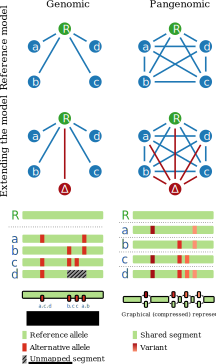
\includegraphics[width=0.9\textwidth]{figures/gen_vs_pang.pdf}
    \centering
    %\caption{}
    %\label{A}
  \end{subfigure}
  \begin{subfigure}[b]{0.5\textwidth}
    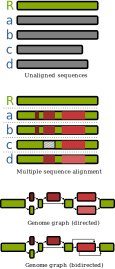
\includegraphics[width=0.9\textwidth]{figures/data_structures.pdf}
    \centering
    %\caption{}
    %\label{B}
  \end{subfigure}
  \\
  \caption{
    \label{fig:models}
    Pangenomic models.
    \emph{Left panel}:
    (top left) In reference based genomic analyses, all genomes ($A \ldots D$) are compared to each other via their relationship to the reference genome $R$.
    (top right) In a pangenomic setting, we attempt to model direct relationships between all the genomes in our analysis, of which a particular reference $R$ is chosen arbitrarily.
    (middle left) When extending our analysis with a new genome, $\Delta$, we add it to the genomic model by comparing it to reference $R$.
    (middle right) In contrast, adding a new genome to a pangenomic analysis compares it directly with all other genomes in the model.
    (bottom left) Regions of some genomes are unalignable against the reference, and cannot be represented in a list of variants.
    (bottom right) A graphical model of the genomes allows direct all-to-all comparison, capturing all of their sequence relationships.
    \emph{Right panel}:
    (top left) A collection of sequences representing a pangenome.
    (top right) Multiple sequence alignment of the sequences captures their mutual relationships.
    (middle top) In a de Bruijn graph, sequences are represented without bias, but variants may correspond to larger graph structures.
    (middle bottom) An acyclic sequence graph is equivalent to the multiple sequence alignment.
    (bottom) A generic sequence graph can represent a structural variant (in orange, right) compactly, using edges between the forward and reverse strands of the graph to indicate the presence of an inversion.
  }
\end{figure}

\begin{figure}[p]
    \includegraphics[width=0.9\textwidth]{figures/visualization.pdf}
    \caption{\label{fig:visualization} An overview of several approaches to visualizing assembly, scaffold, and comprehensive pangenome graphs.
\textbf{A:} Bandage, adapted from \cite{Wick_2015} supplementary section~6.
\textbf{B:} GfaViz, adapted from \cite{Gonnella_2018} supplementary figure~S4.
\textbf{C:} SGTK, adapted from \cite{Kunyavskaya_2018} figure~1.
\textbf{D:} AGB, adapted from \cite{Mikheenko_2019} supplementary figure~S3.
\textbf{E:} Sequence Tube Map, adapted from \cite{Beyer_2019} figure~2.
\textbf{F:} \texttt{vg viz}, adapted from \cite{Garrison_2019} figure~2.20.}
\end{figure}


% TODO: this was in the table but I couldn't find a citation or a web page for it so I cut it.
% SHIMMER Sketch Graph & Force-directed & Variation graphs &  & Command line tool, static images, GraphViz, Gephi \\ \cline{1-3} \cline{5-5}

\begin{table}[p]
\centering
\caption{\label{table:Visualization_Features} An overview of graph visualization tools. \textbf{FD}~=~Force-directed layout, \textbf{SM}~=~Sorted-matrix layout, \textbf{A}~=~Assembly graph, \textbf{S}~=~Scaffold graph, \textbf{V}~=~Variation graph, \textbf{B}~=~Base-level view, \textbf{L}~=~Linear view, \textbf{UI}~=~User interface, \textbf{App}~=~native application, \textbf{Web}~=~browser-based interface, \textbf{CLI}~=~command-line tool.}
\vspace{4mm}
\begin{minipage}{1.0\textwidth}
\begin{tabular}{|l|c|c|c|c|c|p{2.2cm}|}
\hline
\textbf{Tool} & \textbf{Layout} & \textbf{\twoline{Graph}{Type}} & \textbf{\twoline{Proven}{Scale}} & \textbf{\twoline{Extra}{Views}} & \textbf{UI} & \textbf{Backend} \\
\hline
Bandage \cite{Wick_2015} & FD & A & 100~Mbp & & App & \\
\hline
GfaViz \cite{Gonnella_2018} & FD & A, V & 1~Mbp & & App & OGDF \cite{Chimani_2012_OGDF} \\
\hline
SGTK \cite{Kunyavskaya_2018} & FD & A, S & 1~Mbp & B, L & Web &  \texttt{cytoscape.js} \cite{Franz_2016_cytoscape} \\
\hline
AGB  \cite{Mikheenko_2019} & Rank & A & 10k edges\footnote{\url{https://github.com/almiheenko/almiheenko.github.io/blob/8f4b2f8c/AGB/Flye_Human/data/repeat_graph.json}} & L & Web & \texttt{d3-graphviz}\footnote{\url{https://github.com/magjac/d3-graphviz}} \\
\hline
\twoline{Sequence Tube}{Map \cite{Beyer_2019}} & Tube & V & 100~Mbp & B, L & Web & \\
\hline
MoMI-G \cite{yokoyama_momi-g:_2019} & \twoline{Tube\cite{Beyer_2019},}{Circos\cite{Krzywinski_2009_Circos}}  & V & 1~Gbp & B, L & Web & Sequence Tube Map, Circos \\
\hline
\texttt{vg view} \cite{Garrison_2018} & Rank & V & 10~Kbp & B & CLI & GraphViz \\
\hline
\texttt{vg viz} \cite{Garrison_2019} & SM & V & 100~Kbp & B, L & CLI & \\
\hline
\texttt{odgi viz} & SM & V & 1~Gbp & B, L & CLI & \\
\hline
\end{tabular}
\end{minipage}
\end{table}




\begin{table}[h!]
\centering
\caption{An overview of graph mapping tools}
\vspace{10mm}
\label{table:mappers}
\begin{tabular}{|p{2.25cm}|p{2.5cm}|p{1.75cm}|p{2.5cm}|}
 \hline
 \textbf{Tool} & \textbf{Graph Types} & \textbf{Sequencing Types} & \textbf{Other Notes} \\
 \hline
 \hline
deBGA & \multirow[c]{3}{=}{De Bruijn graph} & \multirow[c]{3}{=}{NGS} &  \\ \cline{1-1} \cline{4-4}
BGREAT &  &  & Gapless alignment  \\ \cline{1-1} \cline{4-4}
BrownieAligner &  &  &   \\ \hline
GenomeMapper & \multirow[c]{4}{=}{Acyclic variation graph} & \multirow[c]{3}{=}{NGS} & No longer maintained \\ \cline{1-1} \cline{4-4}
Graph Genome Aligner &  &  &  \\ \cline{1-1} \cline{4-4}
HISAT2 &  &  & Fast \\ \cline{1-1} \cline{3-4}
V-MAP &  & NGS and long read & \\ \hline
VG & Variation graph & NGS and long read & Accurate, high memory usage \\ \hline
GraphAligner & Variation graph or overlap graph & Long read & Fast \\ \hline
%GfaViz &  & assembly graphs, variation graphs & \multirow{15}{=}{megabase subgraph of a variation graph, no nucleotide level} & interactive desktop app, GFA2 support, OGDF\cite{Chimani_2012_OGDF} \\ \cline{1-1} \cline{3-3} \cline{5-5}
%SHIMMER Sketch Graph &  & variation graphs &  & cli app, static images, GraphViz, Gephi \\ \cline{1-3} \cline{5-5}
%SGTK & \multirow{10}{=}{force-directed, genome browser mode} & scaffold graphs, assembly graphs, reads, reference sequences &  & interactive web app, cytoscape.js\cite{Franz_2016_cytoscape} \\ \cline{1-1} \cline{3-5}
%AGB &  & assembly graphs, reference sequences & topological complexity: thousands of edges\footnote{\url{https://github.com/almiheenko/almiheenko.github.io/blob/8f4b2f8c7c498f04fa32f53f69b4bc59888a14f0/AGB/Flye_Human/data/repeat_graph.json}} & interactive web app, d3-graphviz\footnote{\url{https://github.com/magjac/d3-graphviz}} \\\hline
%SequenceTubeMap & pseudo-linear tubemap & \multirow{23}{=}{variation graphs} & from nucleotides to kilobases & interactive web app, unique layout \\ \cline{1-2} \cline{4-5}
%MoMI-G & pseudo-linear tubemap, circos, linear annotation &  & gigabase circos, from nucleotides to kilobases & interactive web app, multiple views \\ \cline{1-2} \cline{4-5}
%vg view & force-directed &  & 10 kilobase subgraph of a variation graph, nucleotide resolution & cli app, static image, GraphViz\\ \cline{1-2} \cline{4-5}
%vg viz & \multirow{7}{=}{rectangular sorted matrix} &  & 100 kilobase subgraph of a variation graph & cli app, static image \\ \cline{1-1} \cline{4-5}
%odgi viz &  &  & from nucleotide resolution to gigabase genomes & cli app, static image, binning \\\hline
\end{tabular}
\end{table}


% References
%
% Margin notes within bibliography

\noindent
\bibliography{bib/references.bib}

%To download the appropriate bibliography style file, please see \url{http://www.annualreviews.org/page/authors/author-instructions/preparing/latex}. 


%Please see the Style Guide document for instructions on preparing your Literature Cited.

%The citations should be numbered in alphabetical order, with titles. For example:



\end{document}
